\documentclass[USenglish,pdftex,compress,10pt,svgnamesi,handout]{beamer}
%\documentclass[USenglish,pdftex,compress,10pt,svgnames]{beamer}
\usepackage{import}\subimport{../../common/}{lectureheader}

\graphicspath{{pics/}}
\usepackage{listings}

\parskip2ex
\usepackage{tabu}

\newcommand{\bfw}{\Vec{w}}
\newcommand{\bfx}{\Vec{x}}
\newcommand{\bfz}{\Vec{z}}
\newcommand{\bfg}{\Vec{g}}
\newcommand{\bfu}{\Vec{u}}
\def\bf#1{\Vec{#1}}
\def\cl#1{{\cal #1}}
\DeclareMathOperator{\sgn}{sgn}
\def\hid{{H}}


% =====================================================================
% Titel etc.
\hypersetup{%
	pdftitle={neural networks: introduction},%
	pdfauthor={Patrick van der Smagt}%
}

\title{neural networks 1:  inverted classroom slides}
\author{Patrick van der Smagt}
\date{}
% =====================================================================
\begin{document}
\lstset{language=Pascal}


%'''''''''''''''''''''''''''''''''''''''''''''''''''''''''
\begin{frame}
	\titlepage
	
	\vfil
\end{frame}









\begin{frame}
    \frametitle{how do we find the best weights in an NN?}

Q: use an optimiser, e.g., CG, Adam, \dots

\pause
Those optimisers work best if they have access to $\partial E / \partial w_{ij}$, the gradient of the loss w.r.t.\ $w_{ij}$.
Back-propagation is the name of the method to compute this gradient.
\end{frame}




\begin{frame}
    \frametitle{why do we use nonlinear activation functions?}


``They serve as an activation function to imitate the biological activation function of a neuron.''\\
``They adapt to the data during the training''\\
``to determine the weight w of the data''\\
``\dots transform data\dots''\\
``\textbf{to introduce nonlinearity}''
\end{frame}

\begin{frame}
    \frametitle{why do we use nonlinear activation functions?}
    
    \begin{align}
    y &= W_n \,\phi( W_{n-1} \,\phi (\dots \,\phi(W_0 X) \dots))\nonumber \\
          &\textcolor{white}{= W_n W_{n-1} \dots W_1 W_0 X}\nonumber\\
                    &\textcolor{white}{= W'X}\nonumber
    \end{align}

\end{frame}


\begin{frame}
    \frametitle{why do we use nonlinear activation functions? }
    
    \begin{align}
        y &= W_n \,\textcolor{white}{\phi}( W_{n-1} \,\textcolor{white}{\phi} (\dots \,\textcolor{white}{\phi}(W_0 X) \dots))\nonumber\\
          &\textcolor{white}{= W_n W_{n-1} \dots W_1 W_0 X}\nonumber\\
          &\textcolor{white}{= W'X}\nonumber
    \end{align}
\end{frame}

\begin{frame}
    \frametitle{why do we use nonlinear activation functions?}
    
    \begin{align}
        y &= W_n \,\textcolor{white}{\phi}( W_{n-1} \,\textcolor{white}{\phi} (\dots \,\textcolor{white}{\phi}(W_0 X) \dots)\nonumber)\\
              &= (W_n W_{n-1} \dots W_1 W_0) X\nonumber\\
          &\textcolor{white}{= W'X}\nonumber
    \end{align}
\end{frame}

\begin{frame}
    \frametitle{why do we use nonlinear activation functions?}
    
    \begin{align}
        y &= W_n \,\textcolor{white}{\phi}( W_{n-1} \,\textcolor{white}{\phi} (\dots \,\textcolor{white}{\phi}(W_0 X) \dots)\nonumber)\\
              &= (W_n W_{n-1} \dots W_1 W_0) X\nonumber\\
                        &= W'X\nonumber
    \end{align}
\end{frame}

\begin{frame}
    \frametitle{why do we use nonlinear activation functions?}

``They can be nonlinear while our optimisation problem stays linear in w.''\\
    \begin{align}
    y &= W_n \,\phi( W_{n-1} \,\phi (\dots \,\phi(W_0 X) \dots))\nonumber \\
          &\textcolor{white}{= W_n W_{n-1} \dots W_1 W_0 X}\nonumber\\
                    &\textcolor{white}{= W'X}\nonumber
    \end{align}

\end{frame}



\begin{frame}
    \frametitle{why neural networks over linear regression?}
    It's all about basis functions.  How do you choose them?  
    
    polynomial: $$\sum_i x^i$$
    
    sigmoid: $$1 \over 1 + \exp(-c x)$$
    	$$\tanh(cx)$$
    
    Gaussian: $$\exp(-c x^2)$$
    
    RELU, softmax: $$\mathrm{max}(0,x)$$  $$\ln(1+e^x)$$
\end{frame}
 




\begin{frame}
    \frametitle{what is ``deep'' about deep neural networks?}
    \begin{columns}
    \begin{column}{6cm}
    linear regression
    \end{column}
    \begin{column}{6cm}
     \includegraphics[width=2cm]{pics/nn0l}
    \end{column}
    \end{columns}   
    
     \begin{columns}
    \begin{column}{6cm}
    neural network with 1 hidden layer\\
    don't say: NN with 2 layers
    \end{column}
    \begin{column}{6cm}
     \includegraphics[width=2cm]{pics/nn1l}
    \end{column}
    \end{columns}    
    
    \begin{columns}
    \begin{column}{6cm}
    neural network with 2 hidden layers\\
    don't say: NN with 3 layers
    \end{column}
    \begin{column}{6cm}
     \includegraphics[width=2cm]{pics/nn2l}
    \end{column}
    \end{columns}
    
\end{frame}


\begin{frame}
    \frametitle{what is ``deep'' about deep neural networks?}
   ``sounds fancy'': a typical Machine Learning disease
 
Some papers use very deep NN, with hundreds of hidden layers (example: Microsoft winning ImageNet in Dec.\ 2015 with 152 hidden layers: \url{https://arxiv.org/abs/1512.03385}).
\end{frame}


\begin{frame}
    \frametitle{why do deep neural networks work better?}

one learns ``features'' of ``features''.  This allows for \textsl{better generalisation}.

A ``wide'' network tends to memorise data.

\includegraphics[width=8cm]{pics/Tmu9G.jpg}
\end{frame}


% use this for invisible text, in particular invisible underbraces
\def\i#1{\textcolor{white}{#1}}

\begin{frame}
\frametitle{but remember the vanishing gradient}
It is usually true that 
$$  \partial E(\bfw) / \partial w_{ij}^{(\hid)}
  \gg
    \partial E(\bfw) / \partial w_{ij}^{(\hid-1)}
$$
i.e., the lower you get in the network, the more the gradient vanishes.

After all,
$$
{\partial E(\bfw)  \over \partial w_{\hid-1,i,j} }
    = \delta_{\hid-1,j} x_i 
    = \sum_l {\underbrace{\textcolor{black}{\delta_{\hid,l}}}_{\mathrm{small}}}
    	\i{\underbrace{{}_l^(}_{\textcolor{black}{\times}}}
	{\underbrace{ \textcolor{black}{w_{Hlk} x_i }}_{\mathrm{small}}}
	\i{\underbrace{=smaller_l^(}_{\textcolor{black}{=\,\,\,\mathrm{smaller!}}}}
$$\end{frame}



\begin{frame}
    \frametitle{Difference between Shifting and Scaling Inputs}
    It's all about weight initialisation to keep $w^T x$ at reasonable values.
    
See \texttt{scaling.ipynb}
\end{frame}



\begin{frame}
    \frametitle{early stopping: where do we stop training?}
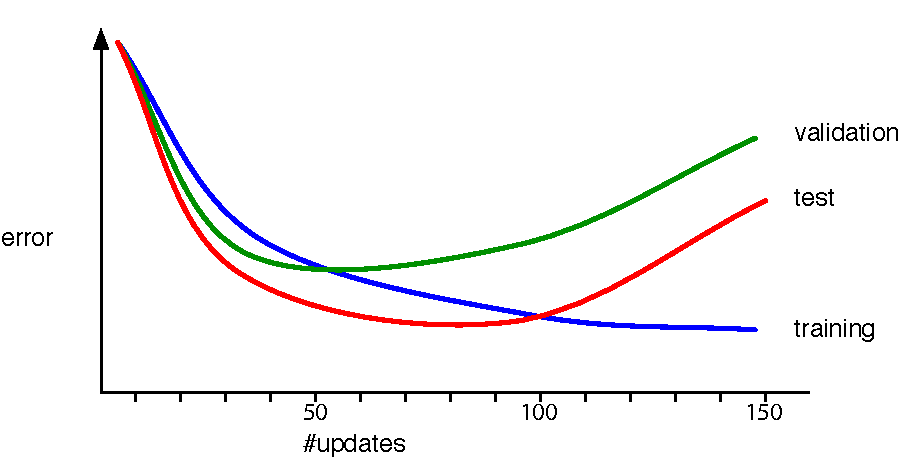
\includegraphics[width=10cm]{pics/train-val-test.pdf}

goal: find the best set of \textsl{hyperparameters} for your model
\end{frame}
\begin{frame}
    \frametitle{early stopping: where do we stop training?}
training set: $\approx$ 60--70\% of the data, \textsl{randomly selected}\\
validation set: $\approx$ 30--20\% of the data,  \textsl{randomly selected}\\
test set: $\approx$ 20--10\% of the data,  \textsl{randomly selected}

\pause randomly selecting data is hard: often subsequent data points are not iid\\[0.5em]
\pause too few data $\rightarrow$ leave-one-out-cross-validation compensates by repeated computation of the result for different data set permutations\\[0.5em]
\pause but \textbf{never ever} report your training error as your result accuracy\\[0.5em]
\pause and please don't report your validation error as your result accuracy
\end{frame}
\begin{frame}
    \frametitle{early stopping: where do we stop training?}
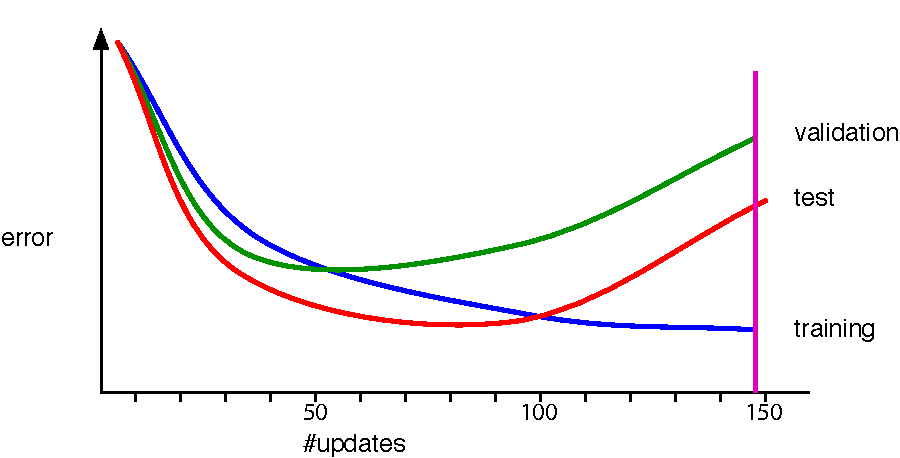
\includegraphics[width=10cm]{pics/train-val-test-1.pdf}

at the lowest training set loss $\Longrightarrow$ bad generalisation
\end{frame}
\begin{frame}
    \frametitle{early stopping: where do we stop training?}
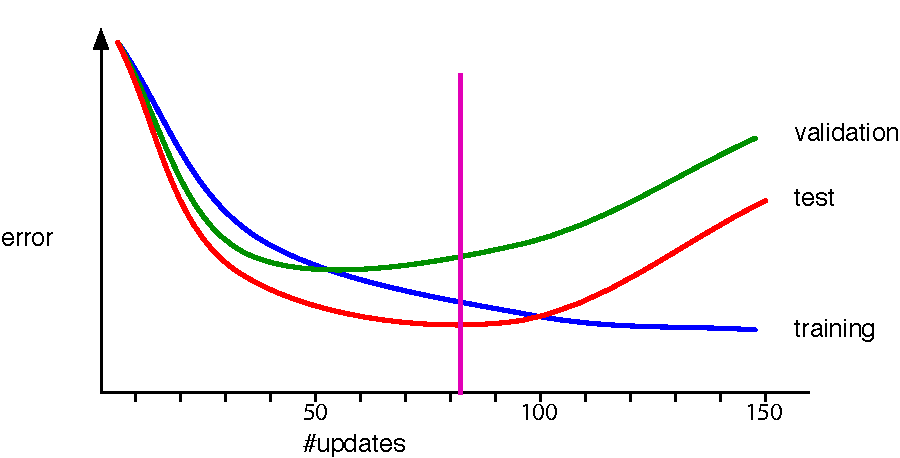
\includegraphics[width=10cm]{pics/train-val-test-3.pdf}

at the lowest test set loss $\Longrightarrow$ bad practice
\end{frame}

\begin{frame}
    \frametitle{early stopping: where do we stop training?}
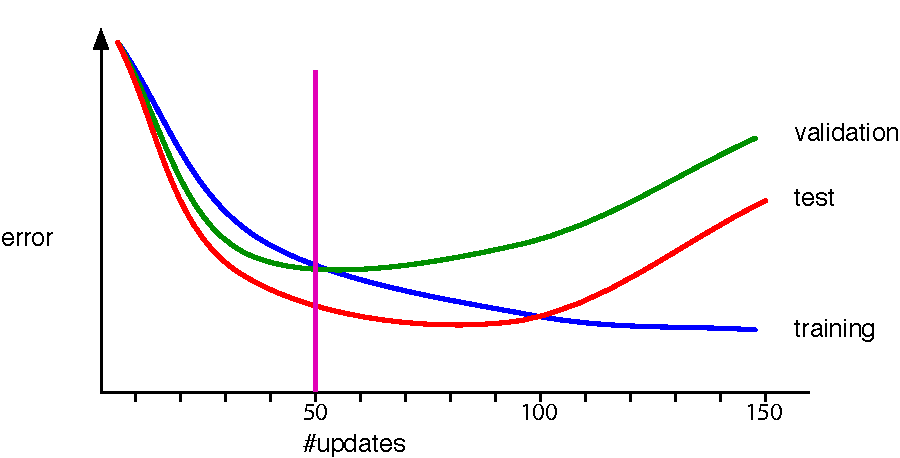
\includegraphics[width=10cm]{pics/train-val-test-2.pdf}

at the lowest validation set loss $\Longrightarrow$ then report your error on the test set
\end{frame}


\begin{frame}
\frametitle{stochastic vs.\ batch training}
We'd prefer to update our parameters after each data point (on-line learning).
But:
\begin{itemize}
\item inefficient computation (think GPU)
\item no tractable way of computing a stable gradient
\end{itemize}

Full batch learning:
\begin{itemize}
\item often does not fit on your GPU
\item leaves out desired stochasticity
\end{itemize}

We therefore usually use mini-batches of size $\approx$ 100--1000
\end{frame}


\end{document}
